

\subsection{Datasets}
For the demonstration, we will use a synthetic tensor and several real-world tensors. We've made stream of a tensor from starting point and split into parts with batch sizes. Here's our datasets and metadata to construct tensor streams.

\begin{table}[htb]
	\small
	\centering
	\begin{tabular}{ c | cccccc }
		\hline
		\textbf{Dataset} & \multicolumn{4}{c}{\textbf{Mode}} & \textbf{Start to Stream} & \textbf{Batch Sizes} \\
		\hline
 		Synthetic Data & 1 K & 10 & 20 & 30 & 5 & 5 * 199\\
 		Sample Video & 205 & 240 & 320 & 3 & 5 & 5 * 40\\
 		Stock & 3 K & 200 & 5 & & 10 & 10 * 299 \\
 		Sever Room CFD & 3 K & 3 & 3 & 34 & 10 & 10 * 299 \\
		\hline
	\end{tabular}
\end{table}

\subsubsection{\em Synthetic Data}
We've constructed synthetic data to manually make temporally changing points. This tensor has its size of $10*20*30*1000$ having the last mode as a temporal mode. The tensor was conducted by concatenation of theme tensor $T$ which is addition of three tensors $T_{main}$, $T_{theme}$ and $T_{noise}$. Each consisting tensor is 100x, 10x and 1x normal distributed randomized tensor respectively and those are used for making different and similar theme tensors.

\begin{table}[htb]
	\small
	\begin{tabular}{ c | cccccccccc }
 		\hline
 		Time Index & 1$\sim$100 & 101$\sim$200 & 201$\sim$250 & 251$\sim$500 & 501$\sim$600 & 601$\sim$700 & 701$\sim$750 & 751$\sim$800 & 801$\sim$950 & 951$\sim$1000 \\
 		\hline
 		Theme & $A$ & $A'$ & $B$ & $B'$ & $B''$ & $C$ & $D$ & $E$ & $E'$ & $E''$ \\
 		\hline
	\end{tabular}
\end{table}

\subsubsection{\em Sample Video}


\subsubsection{\em Stock}
KOSPI200

\subsubsection{\em Server Room CFD}
Temperature was measured in a server room equipped with two heterogeneously occupied racks and one roof-mounted cooling device by 34 probes. 3 servers power usage scenarios and also 3 air conditioning temperature scenarios were performed.

\newpage
\subsection{Experimental Results}
For each dataset, decomposition rank and number of iterations may affect performance of decomposition.
Triggering condition for split and refinement process depends on upper and lower limit of z-score, ${ul}$ and ${ll}$.

\begin{table}[htb]
	\small
	\centering
	\begin{tabular}{ c | cccc }
		\hline
		\textbf{Dataset} & \textbf{Rank} & \textbf{\# of Iterations} & \textbf{${ul}$} & \textbf{${ll}$} \\
		\hline
 		Synthetic Data & 10 & 1 & 1 & 0.5 \\
 		Sample Video & 20 & 1 & 5 & 3 \\
 		Stock & 5 & 5 & 5 & 3 \\
 		Sever Room CFD & 5 & 5 & 3 & 2 \\
		\hline
	\end{tabular}
\end{table}

\subsubsection{\em Sample Video}
\begin{center}
	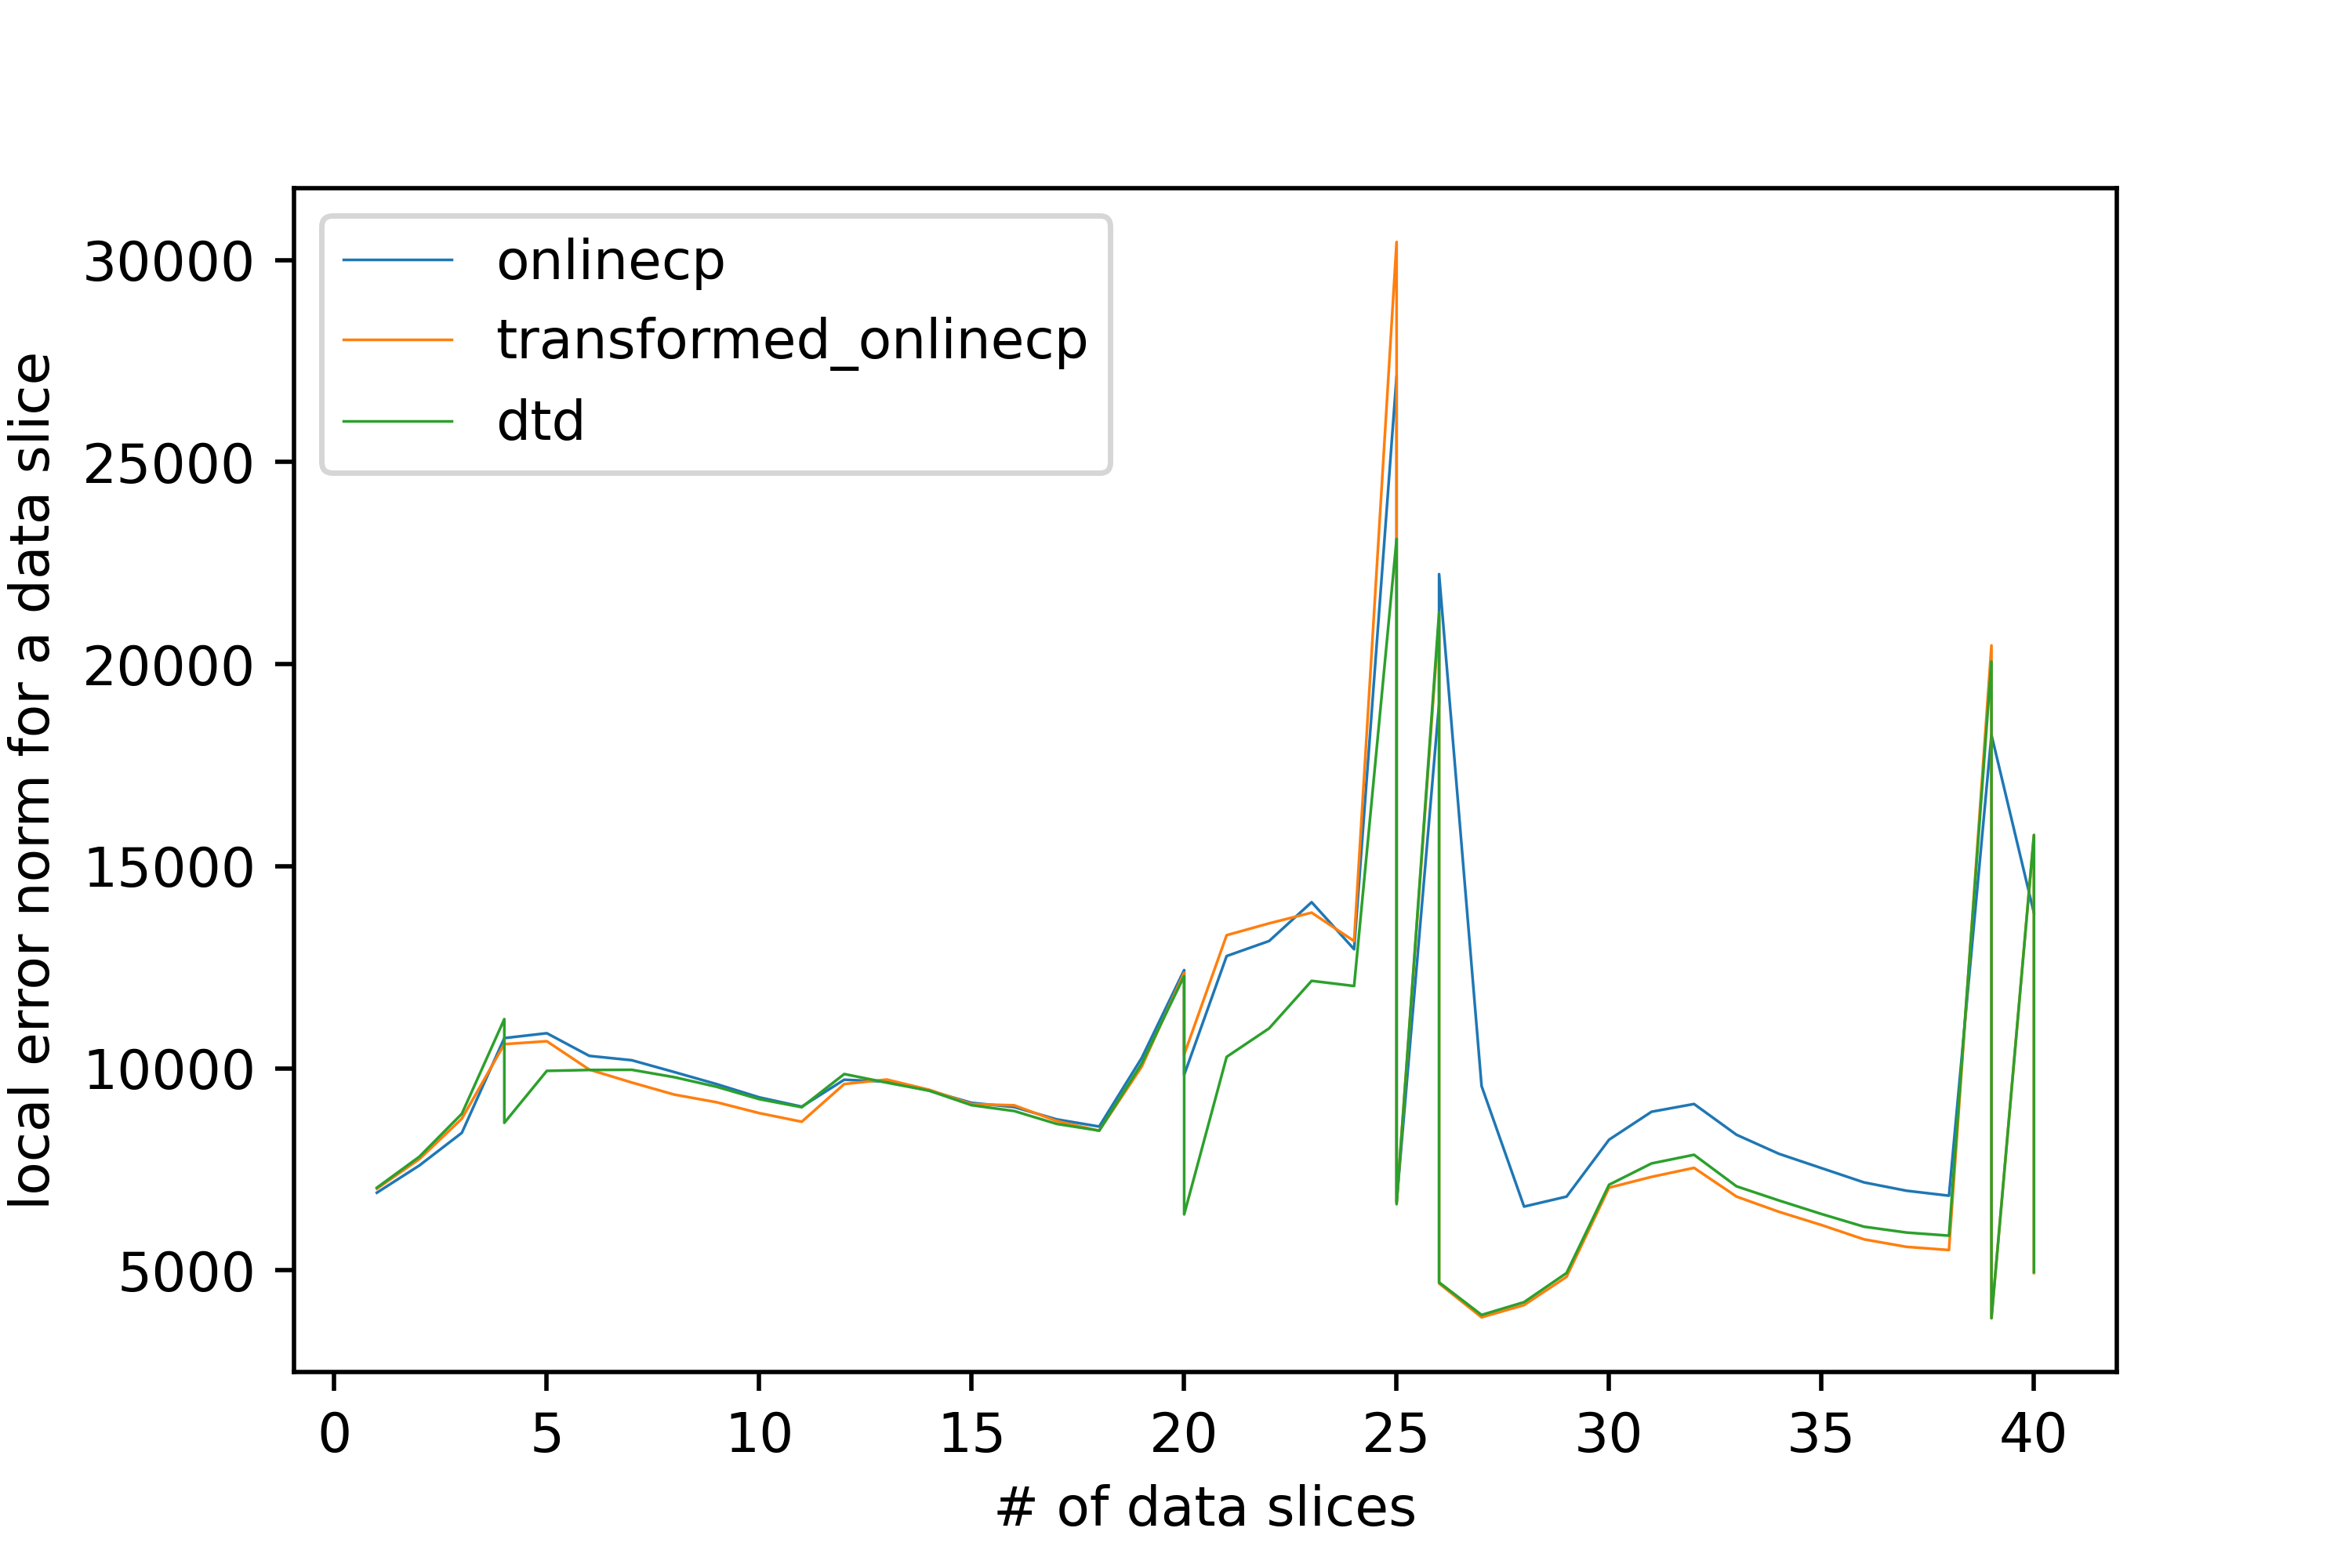
\includegraphics[width=0.49\textwidth]{FIG/sample_video_error_norm.png}
	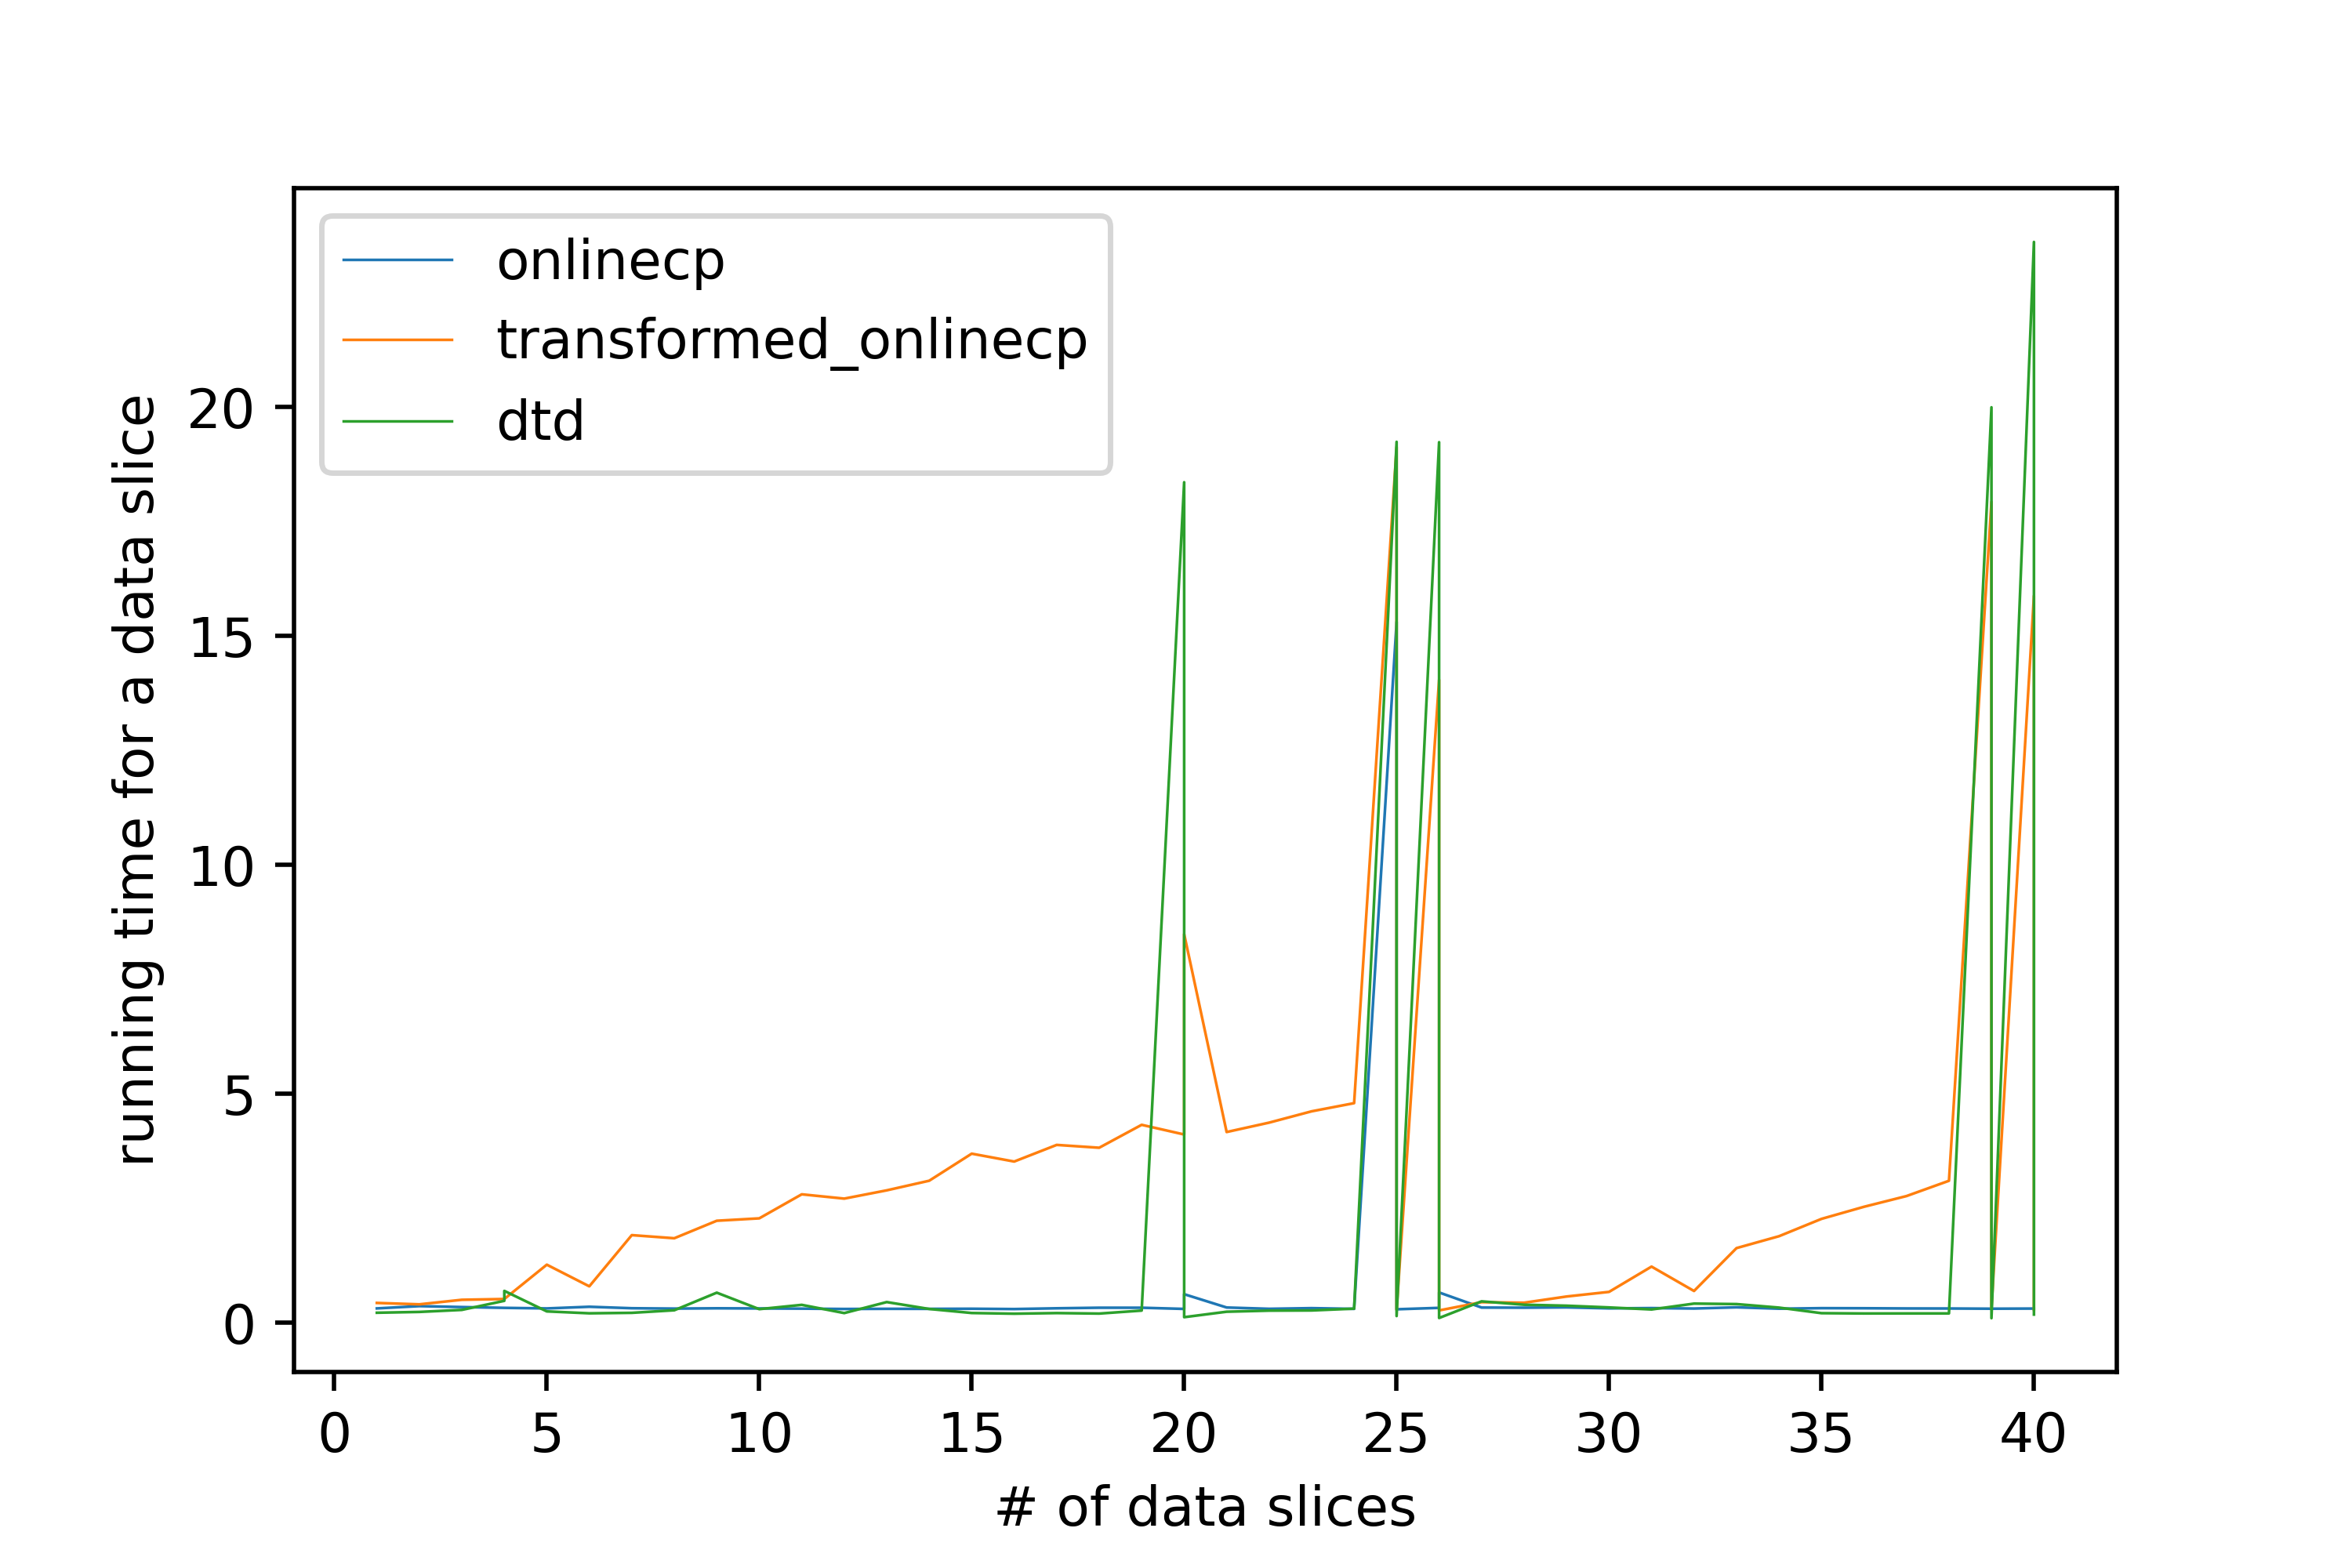
\includegraphics[width=0.49\textwidth]{FIG/sample_video_running_time.png}
\end{center}


\subsubsection{\em Stock}
\begin{center}
	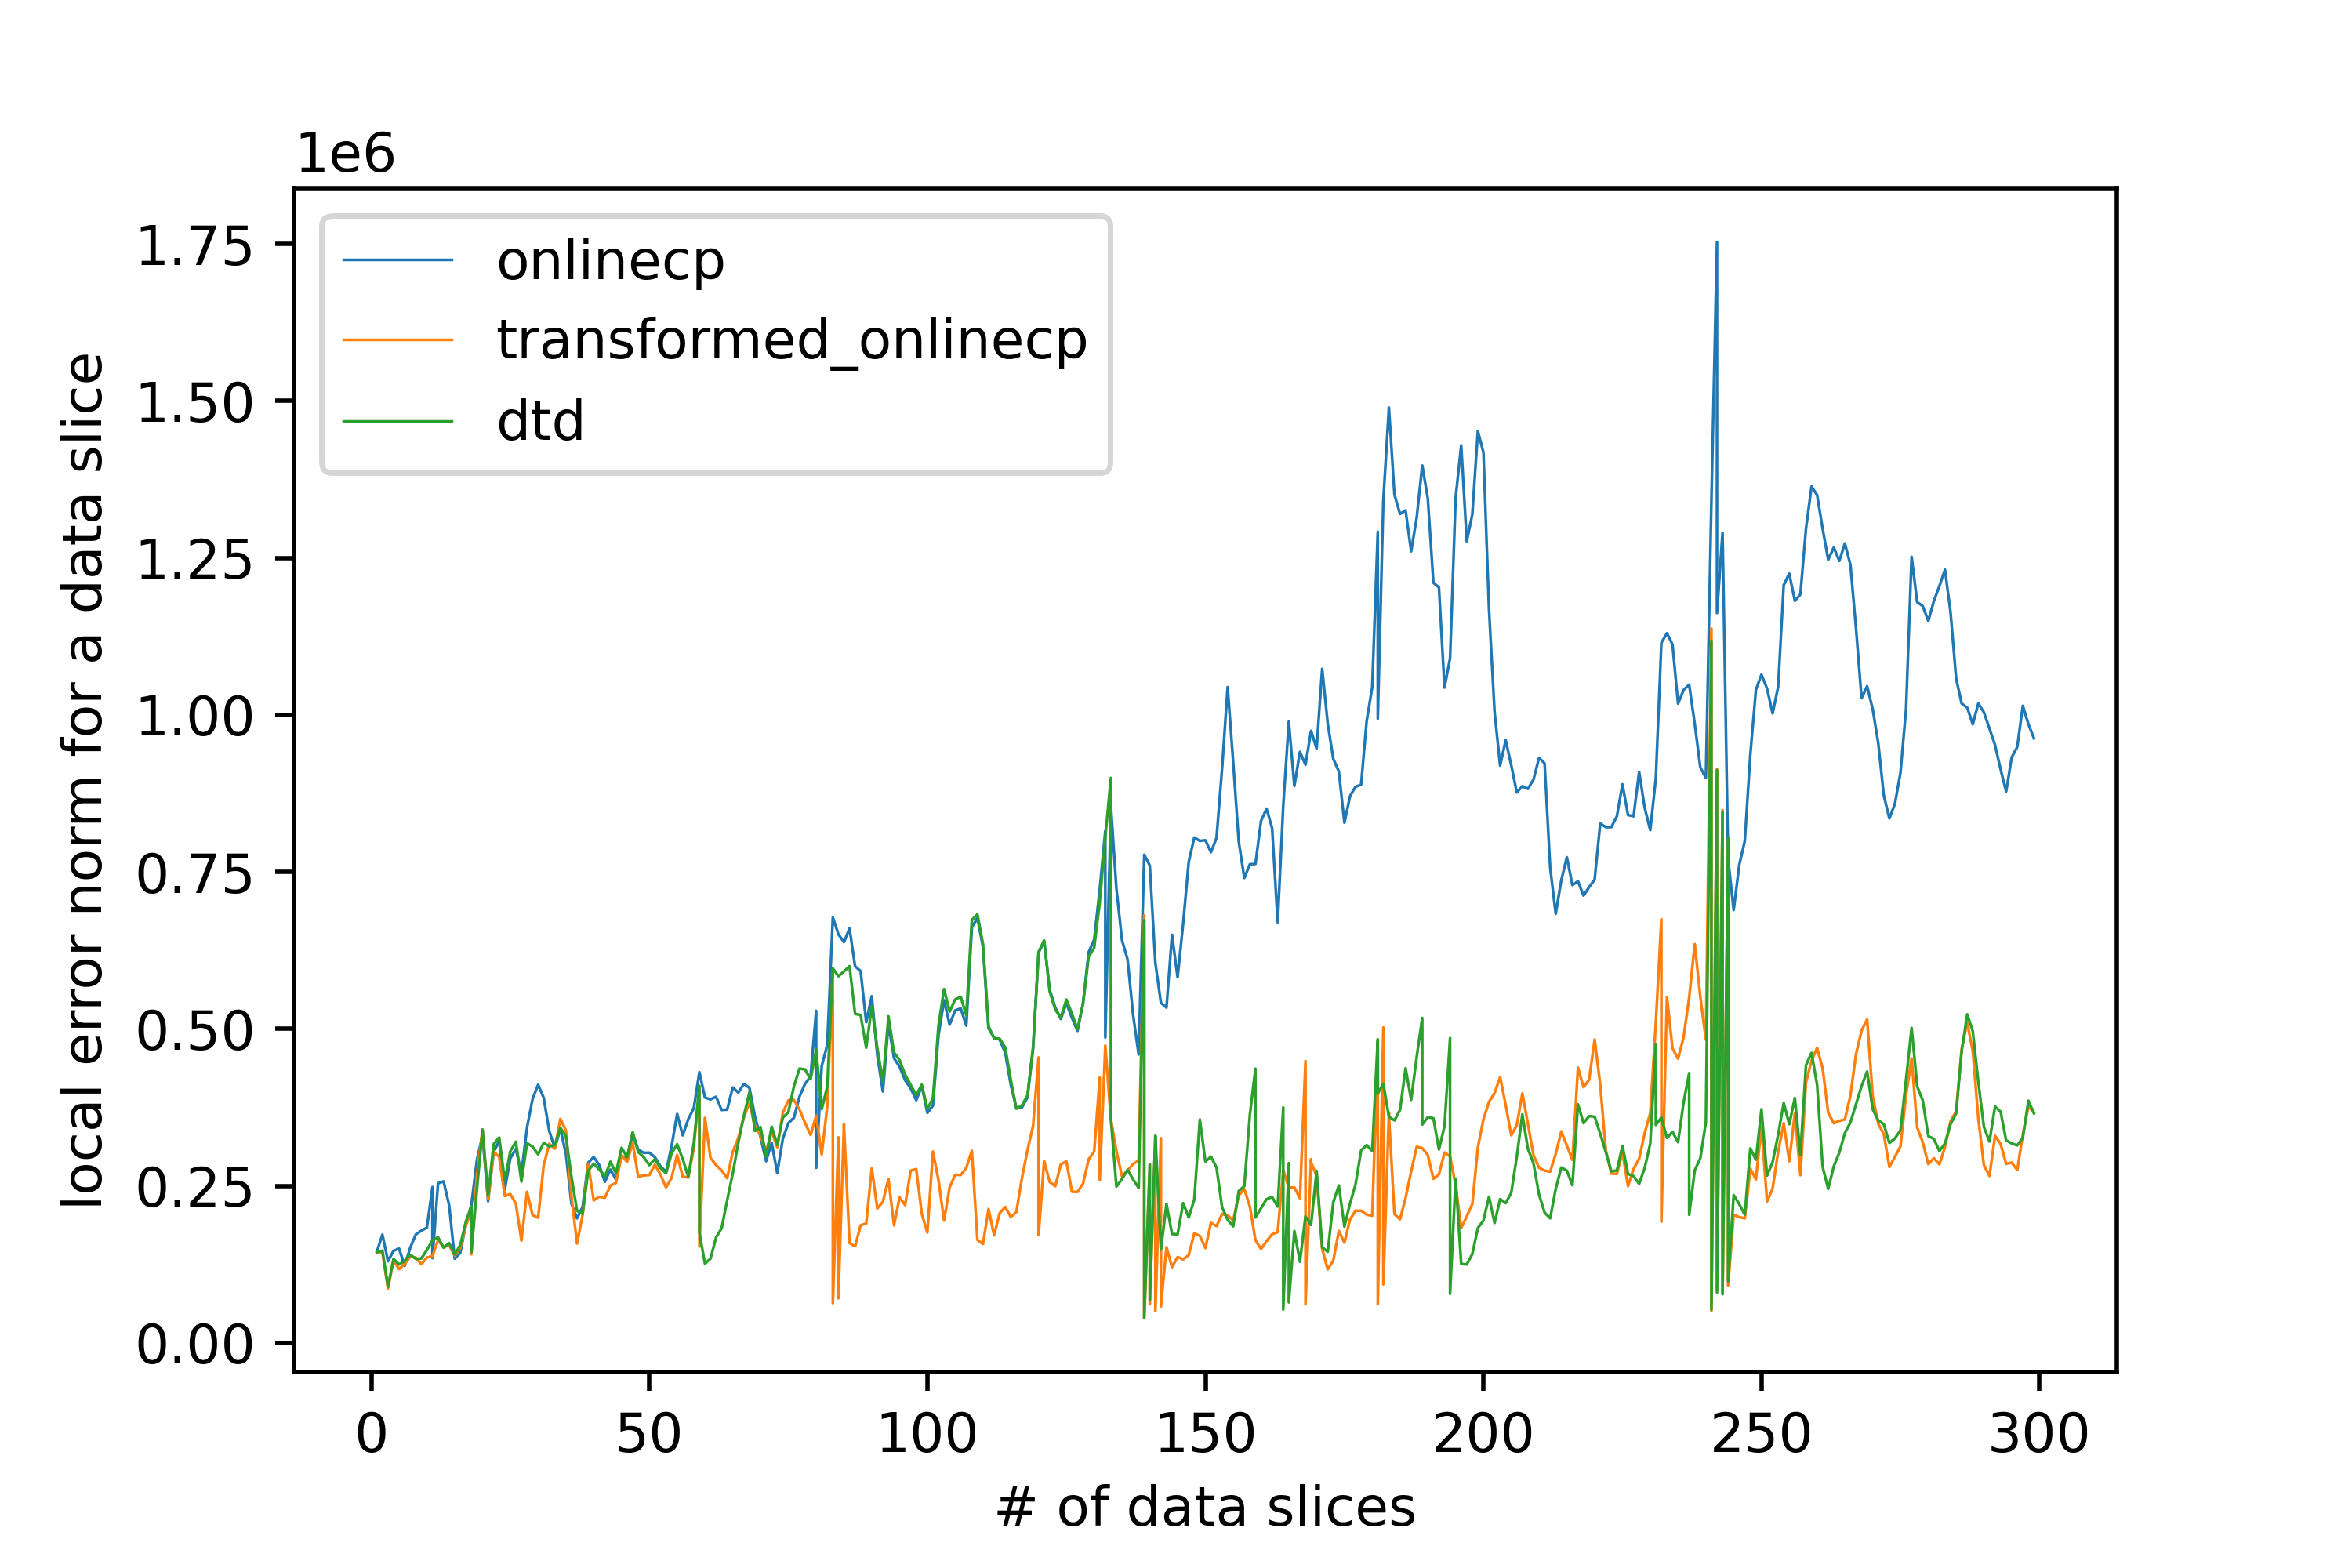
\includegraphics[width=0.49\textwidth]{FIG/stock_error_norm.png}
	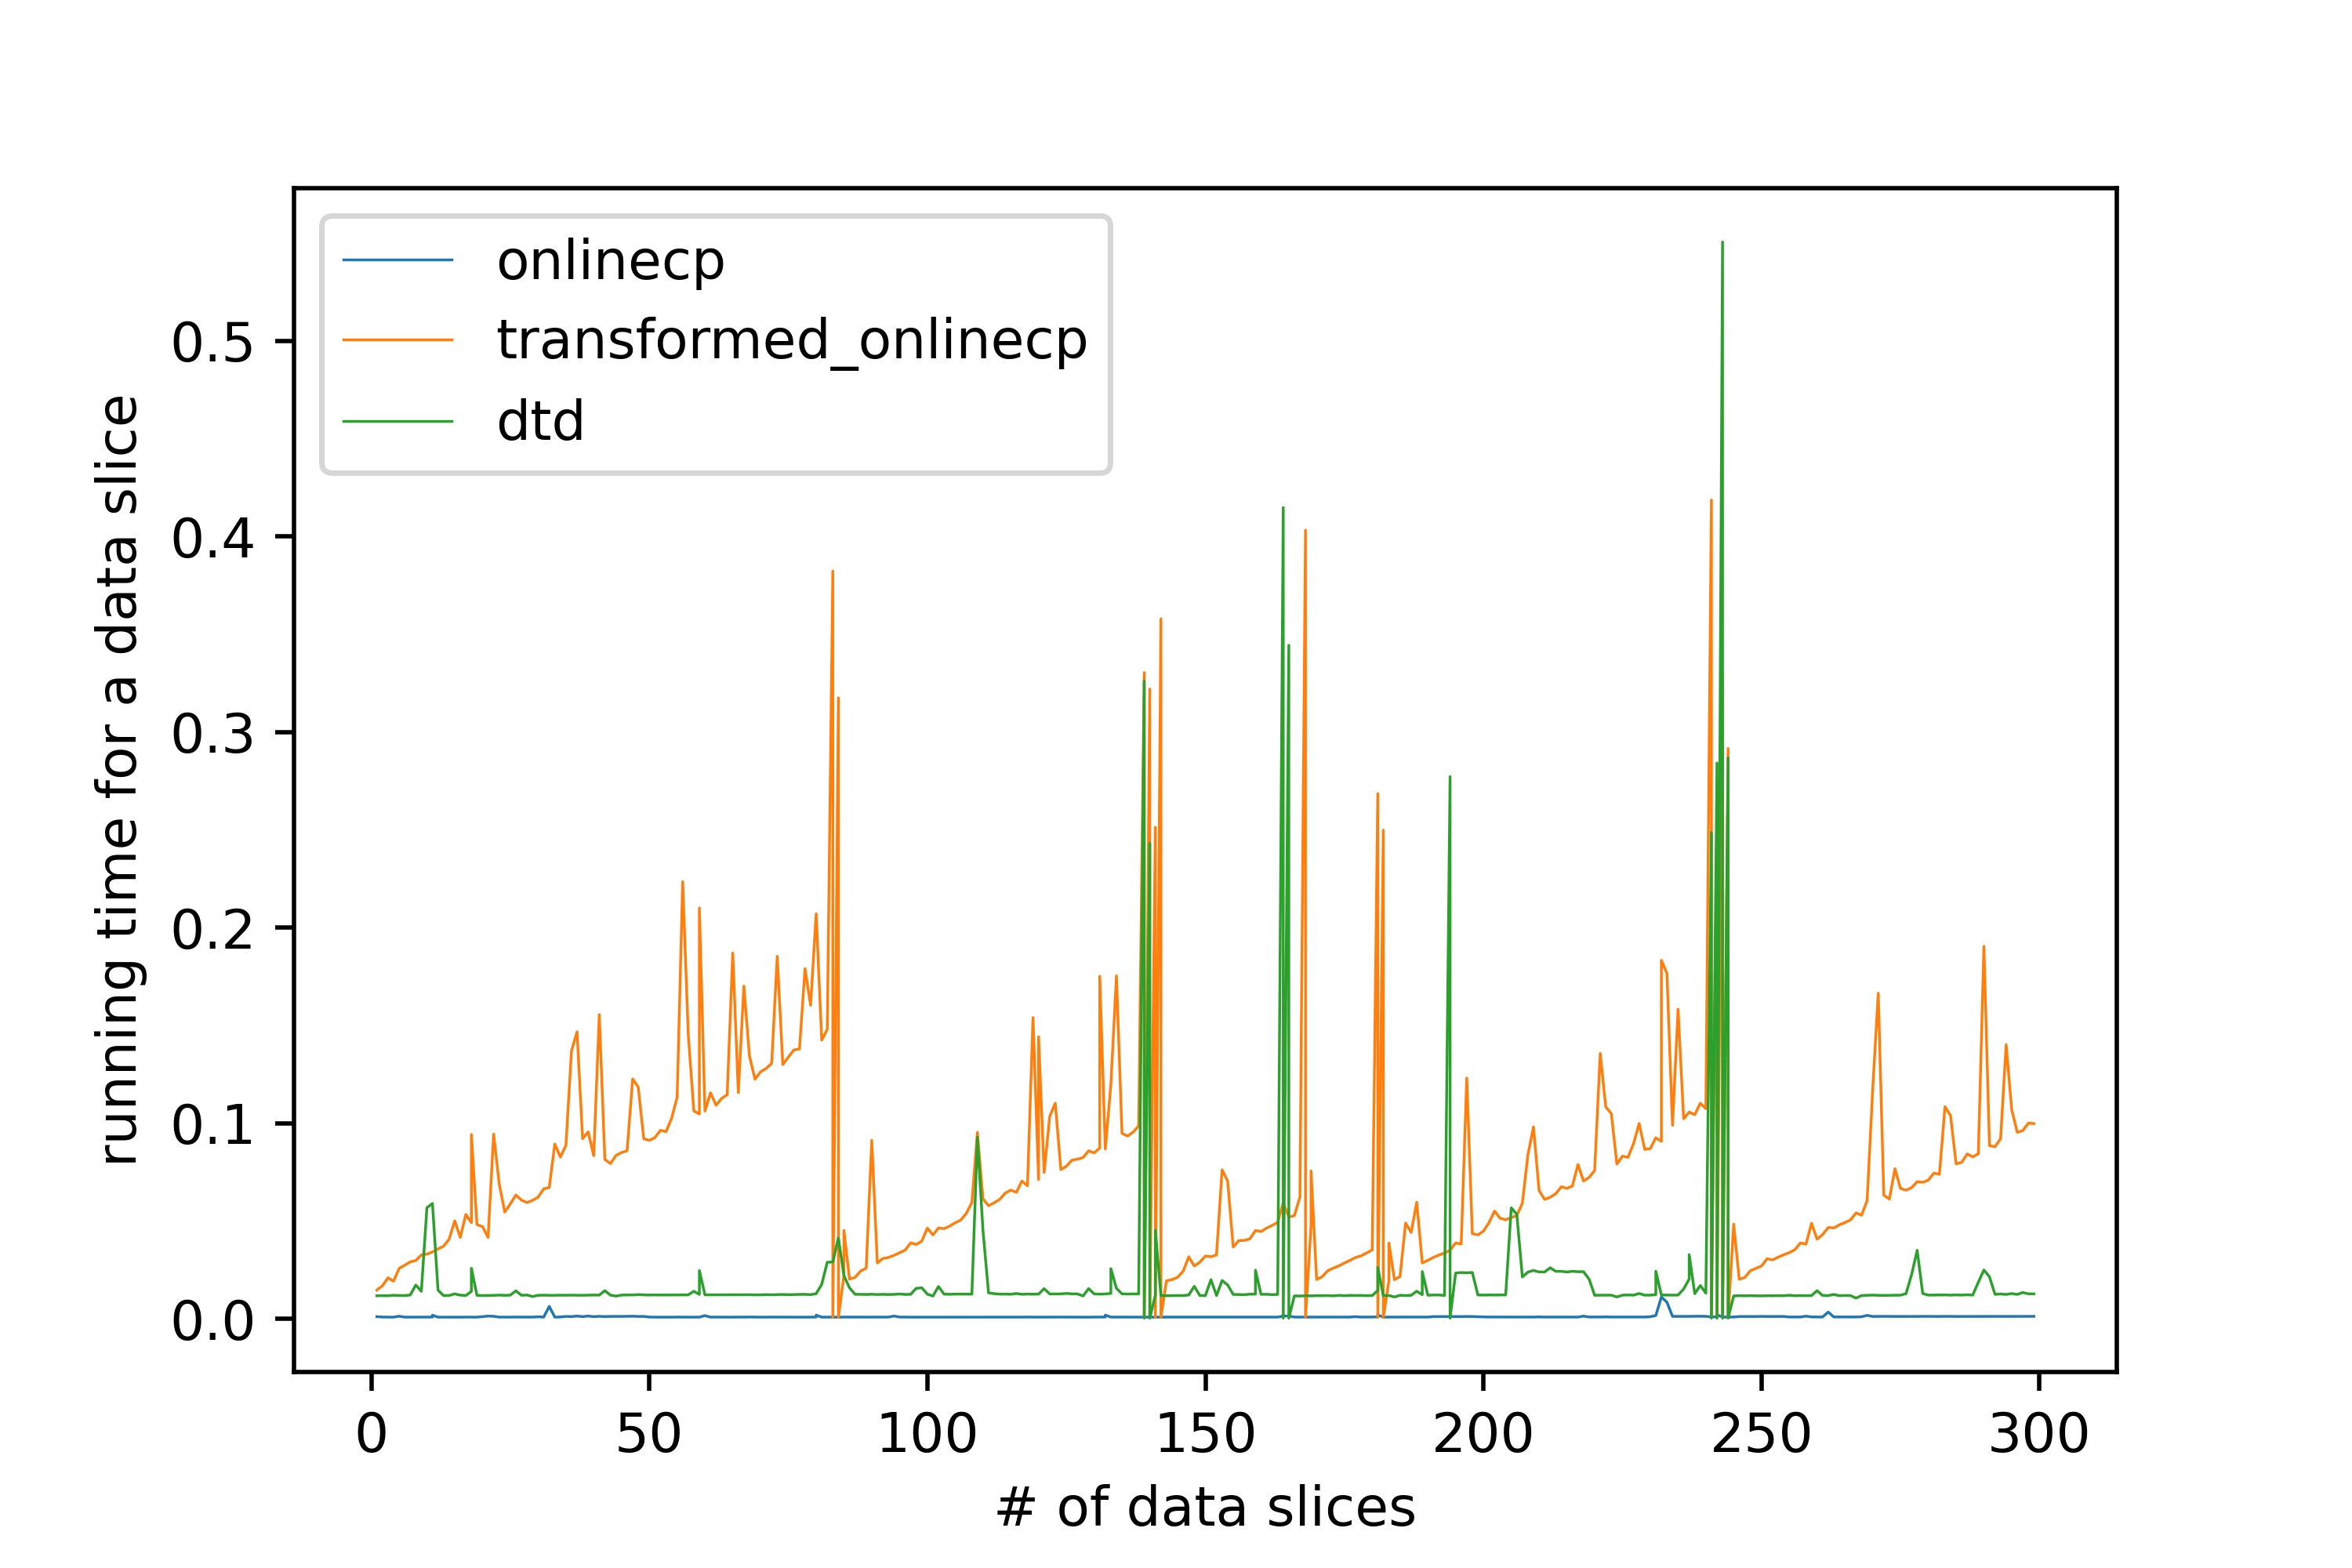
\includegraphics[width=0.49\textwidth]{FIG/stock_running_time.png}
\end{center}
